\documentclass[12pt, a4paper]{report}
\usepackage[margin=1in]{geometry}
\usepackage[utf8]{inputenc}
\usepackage[T1]{fontenc}

\usepackage{times}

\usepackage{float}

\usepackage{url}
\usepackage{graphicx}
\usepackage[colorlinks=false, pdfborder={0 0 0}]{hyperref}

\usepackage{tabularray}

\usepackage{listings}
\usepackage[table, svgnames]{xcolor}
\usepackage[backend=biber, style=alphabetic, sorting=ynt]{biblatex}

% Avoids URLs to overfull \hbox
\usepackage{xurl}

\usepackage{pdfpages}

% Normal table
\colorlet{dark_title_rows}{gray!90}
\colorlet{light_odd_rows}{gray!15}

% Right table
\colorlet{dark_title_rows_right}{teal!90}
\colorlet{light_odd_rows_right}{teal!15}

% Wrong table
\colorlet{dark_title_rows_wrong}{orange!90}
\colorlet{light_odd_rows_wrong}{orange!15}

\definecolor{mysql_comment_green}{rgb}{0.0, 0.5, 0.0}
\definecolor{mysql_keyword_blue}{RGB}{70, 110, 182}
\definecolor{mysql_identifier_chocolate}{RGB}{123, 63, 0}
\definecolor{mysql_function_amber}{RGB}{255, 191, 0}

\lstdefinelanguage{MySQL}{
    morekeywords={
        SELECT, INSERT, UPDATE, DELETE, FROM, WHERE, AND, OR, NOT, CREATE, ALTER, DROP, TABLE, INDEX, VIEW,
        INTO, VALUES, JOIN, INNER, LEFT, RIGHT, ON, GROUP, BY, ORDER, HAVING, AS, DISTINCT, IN, EXISTS,
        BETWEEN, LIKE, IS, NULL, PRIMARY, KEY, FOREIGN, REFERENCES, CONSTRAINT, DATABASE, USE, IF, ELSE,
        END, BEGIN, TRANSACTION, COMMIT, ROLLBACK, GRANT, REVOKE, UNION, ALL, EXCEPT, INTERSECT,
        WITH, PROCEDURE, FUNCTION, TRIGGER, CURSOR, DECLARE, FETCH, OPEN, CLOSE, DEALLOCATE, VARCHAR, INT,
        AUTO_INCREMENT, ENGINE, CHARSET, DEFAULT, TEXT, DATETIME, TIMESTAMP, RECURSIVE, SET
    },
    morekeywords=[2]{
        MAX, MIN, COALESCE, COUNT, SUM, AVG, LENGTH, UPPER, LOWER, CONCAT, NOW
    },
    sensitive=true,
    morecomment=[l]--,
    morecomment=[s]{/*}{*/},
    morestring=[b]',
    morestring=[b]",
    commentstyle=\color{mysql_comment_green}\ttfamily,
    keywordstyle=\color{mysql_keyword_blue}\bfseries,
    keywordstyle=[2]\color{mysql_function_amber},
    literate={?}{{\textcolor{red}{?}}}1,
    stringstyle=\color{gray}\ttfamily,
    identifierstyle=\color{black},
    basewidth={0.5em,0.5em},
    morestring=[b]`,
    stringstyle=\color{mysql_identifier_chocolate}
}

\lstset{
    basicstyle=\ttfamily,                               % Set font type
    keywordstyle=\color{blue}\bfseries,                 % Set keyword color to blue and bold
    stringstyle=\color{red},                            % Set string color to red
    commentstyle=\color{mysql_comment_green}\itshape,   % Set comment color to gray and italic
    breaklines=true,                                    % Enable line breaking
    frame=single,                                       % Add a frame around the code
    numbers=left,                                       % Add line numbers on the left
    numberstyle=\tiny\color{gray},                      % Style for line numbers
    backgroundcolor=\color{lightgray!20},               % Background color
    captionpos=b,                                       % Caption position at the bottom
    showstringspaces=false                              % Don't show spaces in strings
}

% \addbibresource{report.bib}

\graphicspath{{img/}} % global configuration

\title{
    Requirements Manager
    % \begin{figure}[ht]
    % \centering
    % \includegraphics[width=\textwidth]{logo}
    % \end{figure}
}
\author{
    Enrico Marchionni\\
    \texttt{enrico.marchionni@studio.unibo.it}
}
\date{\today}

% Package to keep track of the total number of pages
\usepackage{lastpage}
\usepackage{fancyhdr}

\fancypagestyle{fancy}{
  \fancyhf{}
  \fancyfoot[C]{\thepage\ of \pageref{LastPage}}
  \renewcommand{\headrulewidth}{0pt}
  \renewcommand{\footrulewidth}{0.4pt}
}

\fancypagestyle{plain}{
  \fancyhf{}
  \fancyfoot[C]{\thepage\ of \pageref{LastPage}}
  \renewcommand{\headrulewidth}{0pt}
  \renewcommand{\footrulewidth}{0.4pt}
}

\pagestyle{fancy}

\begin{document}

\maketitle

\begin{abstract}

ReM\footnote{\emph{ReM}, Requirements Manager.} is an administrative software that makes you minimize time and maximize result in
the \emph{Software Engineering} process of collecting and creating requirements.

\end{abstract}

\tableofcontents

\chapter*{Analysis}
\addcontentsline{toc}{chapter}{Analysis}
\label{chap:analysis}

It's requested to realize a database that allows a team to optimize Software's Analysis by managing Requirements creation.
Each one of them descends from a Request that could be created by a team member or by the project customers.

\section*{Interview}
\addcontentsline{toc}{section}{Interview}
\label{sec:interview}

The aim is to manage requirements during all phases of software production and revision storing away all final and in production
data relative to releases already published or yet to publish. Everything has to start from a \emph{Request}.
Once it has been created the relative \emph{Requirement/s} can be developed.

The system admin has to create users and the relative database linked to a software.
Requests can be created by a team member or a customer. Requirements can be developed by team members only. Requests and therefore
Requirements can obviously be added or even edited in later releases. It's not important to keep track of every update or change,
the important is to keep track of final data just before a release. The timeline can be added by a team member only and domain
conditions has to be respected.

Requirements have to be structured with a title, a type (functional, non functional), a version, a description, a body, one or
more files, progress data, a creation time and a last modified time. Moreover for a requirement it has to be known
the user that did the first and last modifications and an history of updates with times and users that did them. Furthermore is
important to consider that requirements could be arranged in a tree structure in the most complex cases.

Requests structure consists of a title, a type, a version, a description, a body, one or more files, a creation time and a last
modified time. Besides for a request it has to be known the user that did the first and last modifications and an history of
updates with times and users that did them.

A requirement has to be associated with one and only one request, a request can be associated with multiple requirements.

A request has to be approved by a team member before developing it into a requirement. After the approval a customer has to
accept the request approval, only then the relative requirement can be developed. When the approval is done the request mustn't
be able to be modified.

Users has to be saved with personal info such as username, name, surname, email, phone and optionally the company name.

The releases should also save a short description and a name that has to be an identifier between the timelines. It's important to
permit the creation of a new timeline only if every requirement was completed, or this mustn't be permitted. In addition every
request has to be approved, formalized into requirement and completed before the version creation.

Every data that was affected by the version cannot be overridden so their last modified time should be previous to the version
creation time.

% There has to be also the possibility to comment (and reply) requests and requirements so as to work in a more interactive and
% efficient way.

\section*{Actions}
\addcontentsline{toc}{section}{Actions}

The mainly requested actions are:
\begin{enumerate}
    \item Subscribe a new user;
    \item View a request;
    \item Create a request;
    \item Update a request;
    \item Approve a request;
    \item View a requirement;
    \item Create a requirement;
    \item Update a requirement;
    \item Disable a requirement;
    \item Create a release;
    \item Show requirements and requests relative to a specific release;
    \item View single requirement history (every change for each release);
    \item Obtain an average of the progress time relative to a branch of the requirements tree;
\end{enumerate}

\chapter*{Design}
\addcontentsline{toc}{chapter}{Design}

\section*{Conceptual Design}
\addcontentsline{toc}{section}{Conceptual Design}

\subsection*{Glossary}
\addcontentsline{toc}{subsection}{Glossary}

A glossary of terms with description, synonyms and links used in \nameref{sec:interview} is here explained in
\autoref{tab:glossary_terms}.

\begin{table}[H]
    \begin{tblr}{
        colspec={X[l]X[l]X[l]X[l]},
        width=\textwidth,
        row{odd}={gray!15},
        row{even}={white},
        row{1}={bg=gray!90,fg=white},
        colsep=4pt
      }
        \textbf{Term} & \textbf{Description} & \textbf{Synonyms} & \textbf{Links} \\
        Request & Customer request of what the system should do & & Requirement, release \\ %, comment \\
        \hline
        Requirement & Formal description of what the system should do & & Request, release \\ %, comment \\
        \hline
        & Requirements + Requests & Data \\
        \hline
        Editor & User that can add Requirements & Team member & \\
        \hline
        Guest & User that can only add Requests & Customer & \\
        \hline
        User & Editor + Guest & User & Editing, versioning \\ %, commenting \\
        \hline
        % Comment & A short text that comments something & Reply & Request, requirement \\
        Release & A timeline that confirms the fact that a software version was released  & Version, timeline & Data \\
        \hline
    \end{tblr}
    \caption{\label{tab:glossary_terms} Glossary of terms}
\end{table}

\subsection*{Requirements}
\addcontentsline{toc}{subsection}{Requirements}

This section aims to restructure requirements according to the \nameref{sec:interview} phase.

\subsubsection*{Functional}

\begin{itemize}
    \item General
    \begin{itemize}
        \item It is demanded to realize a database that manages requirements;
        \item Information that have to be stored are \textbf{Requests}, \textbf{Requirements}, \textbf{Users} and \textbf{Releases}; %and \textbf{Comments};
    \end{itemize}
    \item Users
    \begin{itemize}
        \item \textbf{Users} are structured with username, name, surname, email, phone and optionally the company name;
        \item \textbf{Users} are divided into two groups:
            \begin{itemize}
                \item \textbf{Editors} - they approve \emph{Requests}, develop relative \emph{Requirements} and decides \emph{Releases};
                    in some cases they could also create \emph{Requests};
                \item \textbf{Guests} - they create \emph{Requests} that once approved cannot be edited but will be developed into
                    \emph{Requirements};
            \end{itemize}
    \end{itemize}
    \item Requests
    \begin{itemize}
        \item \textbf{Requests} are structured with a title, a type, a version (positive integer), a description, a body, one or more
            files, a creation time and a last modified time;
    \end{itemize}
    \item Requirements
    \begin{itemize}
        \item \textbf{Requirements} are structured with a title, a type (functional, non functional), a version (positive integer),
            a description, a body, one or more files, progress data (a percentage), a creation time and a last modified time;
        \item \textbf{Requirements} could be arranged in a tree structure;
    \end{itemize}
    % \item Comments
    % \begin{itemize}
    %     \item \textbf{Comments} are structured with a description, the last modified time and the creation time;
    %     \item \textbf{Comments} are relative to \emph{Requests} and \emph{Requirements}; \emph{Editors} can comment both while
    %         \emph{Guests} can work only with \emph{Requests};
    % \end{itemize}
    \item Releases
    \begin{itemize}
        \item \textbf{Releases} are structured with a unique name (software version name), a short description and the creation time;
        \item \textbf{Releases} are timelines that can be created only if all \emph{Requests} had been approved and converted into
            already fully developed \emph{Requirements};
    \end{itemize}
    \item Conditions
    \begin{itemize}
        \item all \textbf{Requests} and \textbf{Requirements} relative to a \textbf{Release} have to be historicized;
        \item \textbf{Requests} and \textbf{Requirements} could be modified or even invalidated in later \textbf{Releases};
        \item a \textbf{Requirement} has to be associated with one and only one \textbf{Request}, a \textbf{Request} can be associated
            with multiple \textbf{Requirements}.
    \end{itemize}
\end{itemize}

\subsubsection*{Non-Functional}

\begin{itemize}
    \item Data access has to be really fast;
    \item CRUD\footnote{\emph{CRUD}, Create, read, update, delete.} operations should be non blocking in final
        GUI\footnote{\emph{GUI}, Graphical user interface.};
\end{itemize}

\subsection*{E-R diagram}
\addcontentsline{toc}{subsection}{E-R diagram}

It was chosen a mixed strategy to build the E-R diagram.

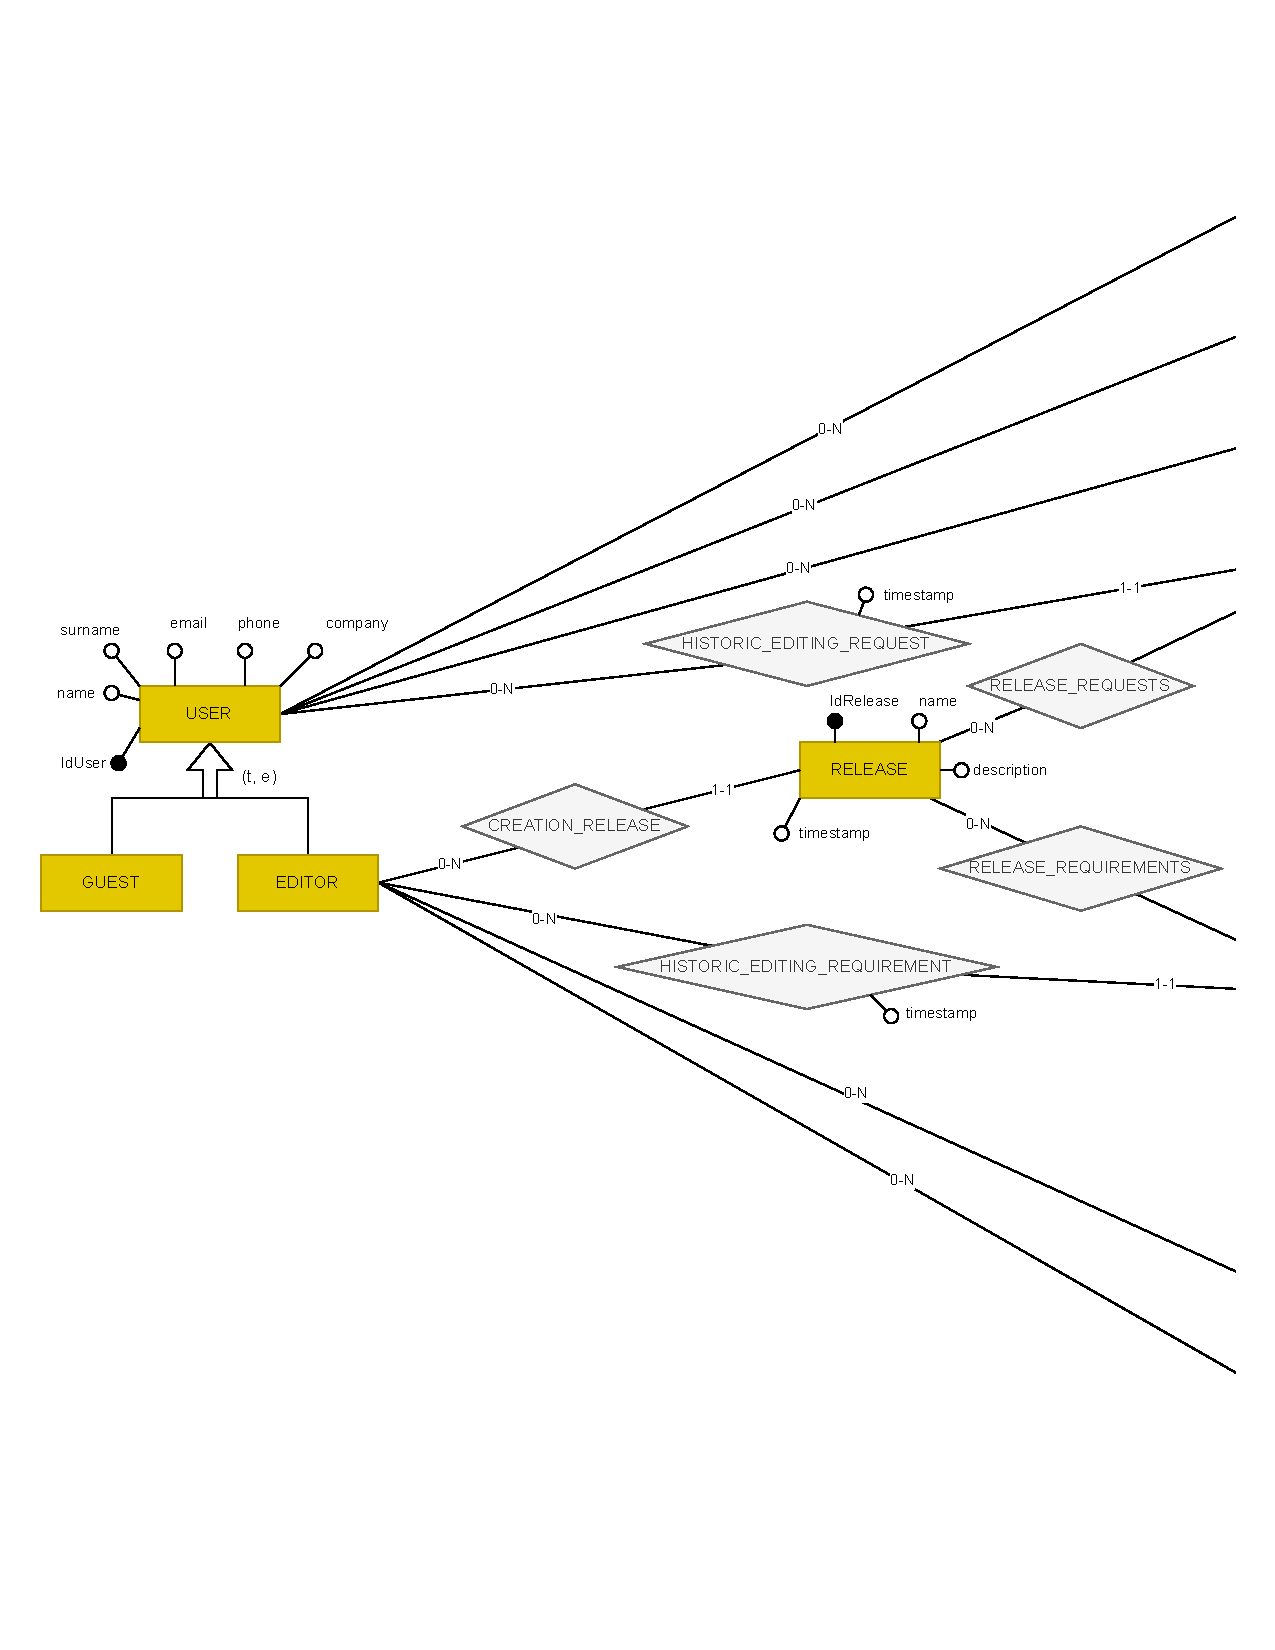
\includepdf[pages=-, pagecommand={\thispagestyle{fancy}}]{E-R}

\section*{Logical Design}
\addcontentsline{toc}{section}{Logical Design}

\subsection*{Table of volumes}
\addcontentsline{toc}{subsection}{Table of volumes}

Data and expected volumes are described in \autoref{tab:volumes_data}.

\begin{table}[H]
    \begin{tblr}{
        colspec={X[l]cc},
        width=\textwidth,
        row{odd}={light_odd_rows},
        row{even}={white},
        row{1}={bg=dark_title_rows,fg=white},
        colsep=4pt
      }
        \textbf{Concept} & \textbf{Construct} & \textbf{Volume} \\
        USER & E & 100 \\
        \hline
        GUEST & E & 90 \\
        \hline
        EDITOR & E & 10 \\
        \hline
        REQUEST & E & 50 \\
        \hline
        HISTORIC\_REQUEST & E & 40 \\
        \hline
        REQUIREMENT & E & 75 \\
        \hline
        HISTORIC\_REQUIREMENT & E & 50 \\
        \hline
        RELEASE & E & 5 \\
        \hline
        DEVELOPMENT & R & 70 \\
        \hline
        HISTORIC\_DEVELOPMENT & R & 50 \\
        \hline
        KINSHIP & R & 5 \\
        \hline
        HISTORIC\_KINSHIP & R & 5 \\
        \hline
        CREATION\_RELEASE & R & 5 \\
        \hline
        RELEASE\_REQUESTS & R & 40 \\
        \hline
        RELEASE\_REQUIREMENTS & R & 50 \\
        \hline
        CREATION\_REQUEST & R & 50 \\
        \hline
        EDITING\_REQUEST & R & 50 \\
        \hline
        HISTORIC\_EDITING\_REQUEST & R & 40 \\
        \hline
        APPROVAL\_REQUEST & R & 45 \\
        \hline
        CREATION\_REQUIREMENT & R & 70 \\
        \hline
        EDITING\_REQUIREMENT & R & 70 \\
        \hline
        HISTORIC\_EDITING\_REQUIREMENT & R & 50 \\
        \hline
        ORIGINAL\_REQUEST & R & 40 \\
        \hline
        ORIGINAL\_REQUIREMENT & R & 50 \\
        \hline
    \end{tblr}
    \caption{\label{tab:volumes_data} Volumes of data}
\end{table}

\subsection*{Operations and frequency}
\addcontentsline{toc}{subsection}{Operations and frequency}

Operations and frequency are described in \autoref{tab:op_fr}.

\begin{table}[H]
    \begin{tblr}{
        colspec={rX[l]c},
        width=\textwidth,
        row{odd}={light_odd_rows},
        row{even}={white},
        row{1}={bg=dark_title_rows,fg=white},
        colsep=4pt
      }
        \textbf{Code} & \textbf{Operation} & \textbf{Frequency} \\
        1 & \hyperref[subsubsec:op1]{Subscribe a new user} & 10 every month \\
        \hline
        2 & \hyperref[subsubsec:op2]{View a request} & 200 every day \\
        \hline
        3 & \hyperref[subsubsec:op3]{Create a request} & 2 every day \\
        \hline
        4 & \hyperref[subsubsec:op4]{Update a request} & 5 every day \\
        \hline
        5 & \hyperref[subsubsec:op5]{Approve a request} & 1 every day \\
        \hline
        6 & \hyperref[subsubsec:op6]{View a requirement} & 200 every day \\
        \hline
        7 & \hyperref[subsubsec:op7]{Create a requirement} & 2 every day \\
        \hline
        8 & \hyperref[subsubsec:op8]{Update a requirement} & 50 every day \\
        \hline
        9 & \hyperref[subsubsec:op9]{Disable a requirement} & 1 every month \\
        \hline
        10 & \hyperref[subsubsec:op10]{View a release} & 2 every day \\
        \hline
        11 & \hyperref[subsubsec:op11]{Create a release} & 2 every year \\
        \hline
        12 & \hyperref[subsubsec:op12]{Show requirements and requests relative to a specific release} & 50 every day \\
        \hline
        13 & \hyperref[subsubsec:op13]{View single requirement history (every change for each release)} & 10 every day \\
        \hline
        14 & \hyperref[subsubsec:op14]{Obtain an average of the progress time relative to a branch of the requirements tree} & 20 every day \\
        \hline
    \end{tblr}
    \caption{\label{tab:op_fr} Operations and frequency}
\end{table}

\subsection*{Navigation and access}
\addcontentsline{toc}{subsection}{Navigation and access}
\label{subsec:ops}

\subsubsection*{1. Subscribe a new user}
\label{subsubsec:op1}

User subscription described in \autoref{tab:usr_sub}.

\begin{table}[H]
    \begin{tblr}{
        colspec={lcX[l]c},
        width=\textwidth,
        row{odd}={light_odd_rows_right},
        row{even}={white},
        row{1}={bg=dark_title_rows_right,fg=white},
        row{3}={bg=dark_title_rows_right,fg=white},
        colsep=4pt
      }
        \textbf{Concept} & \textbf{Construct} & \textbf{Access} & \textbf{Type} \\
        User & E & 1 & W \\
        & & Total: 1W $\rightarrow$ 10 every month & \\
    \end{tblr}
    \caption{\label{tab:usr_sub} Subscribe a new user}
\end{table}

\subsubsection*{2. View a request}
\label{subsubsec:op2}

Request visualization described in \autoref{tab:vw_request}.

\begin{table}[H]
    \begin{tblr}{
        colspec={lcX[l]c},
        width=\textwidth,
        row{odd}={light_odd_rows_right},
        row{even}={white},
        row{1}={bg=dark_title_rows_right,fg=white},
        row{3}={bg=dark_title_rows_right,fg=white},
        colsep=4pt
      }
        \textbf{Concept} & \textbf{Construct} & \textbf{Access} & \textbf{Type} \\
        Request & E & 1 & R \\
        & & Total: 1R $\rightarrow$ 200 every day & \\
    \end{tblr}
    \caption{\label{tab:vw_request} View a request}
\end{table}

\subsubsection*{3. Create a request}
\label{subsubsec:op3}

Request creation described in \autoref{tab:cr_request}.

\begin{table}[H]
    \begin{tblr}{
        colspec={lcX[l]c},
        width=\textwidth,
        row{odd}={light_odd_rows_right},
        row{even}={white},
        row{1}={bg=dark_title_rows_right,fg=white},
        row{3}={bg=dark_title_rows_right,fg=white},
        colsep=4pt
      }
        \textbf{Concept} & \textbf{Construct} & \textbf{Access} & \textbf{Type} \\
        Request & E & 1 & W \\
        & & Total: 1W $\rightarrow$ 2 every day & \\
    \end{tblr}
    \caption{\label{tab:cr_request} Create a request}
\end{table}

\subsubsection*{4. Update a request}
\label{subsubsec:op4}

Request updating described in \autoref{tab:upd_request}.

\begin{table}[H]
    \begin{tblr}{
        colspec={lcX[l]c},
        width=\textwidth,
        row{odd}={light_odd_rows_right},
        row{even}={white},
        row{1}={bg=dark_title_rows_right,fg=white},
        row{4}={bg=dark_title_rows_right,fg=white},
        colsep=4pt
      }
        \textbf{Concept} & \textbf{Construct} & \textbf{Access} & \textbf{Type} \\
        Request & E & 1 & R \\
        Request & E & 1 & W \\
        & & Total: 1R + 1W $\rightarrow$ 10 every day & \\
    \end{tblr}
    \caption{\label{tab:upd_request} Update a request}
\end{table}

\subsubsection*{5. Approve a request}
\label{subsubsec:op5}

Request approval described in \autoref{tab:appr_request}.

\begin{table}[H]
    \begin{tblr}{
        colspec={lcX[l]c},
        width=\textwidth,
        row{odd}={light_odd_rows_right},
        row{even}={white},
        row{1}={bg=dark_title_rows_right,fg=white},
        row{4}={bg=dark_title_rows_right,fg=white},
        colsep=4pt
      }
        \textbf{Concept} & \textbf{Construct} & \textbf{Access} & \textbf{Type} \\
        Request & E & 1 & R \\
        Request & E & 1 & W \\
        & & Total: 1R + 1W $\rightarrow$ 2 every day & \\
    \end{tblr}
    \caption{\label{tab:appr_request} Approve a request}
\end{table}

\subsubsection*{6. View a requirement}
\label{subsubsec:op6}

Requirement visualization described in \autoref{tab:vw_requirement}.

\begin{table}[H]
    \begin{tblr}{
        colspec={lcX[l]c},
        width=\textwidth,
        row{odd}={light_odd_rows_right},
        row{even}={white},
        row{1}={bg=dark_title_rows_right,fg=white},
        row{3}={bg=dark_title_rows_right,fg=white},
        colsep=4pt
      }
        \textbf{Concept} & \textbf{Construct} & \textbf{Access} & \textbf{Type} \\
        Requirement & E & 1 & R \\
        & & Total: 1R $\rightarrow$ 200 every day & \\
    \end{tblr}
    \caption{\label{tab:vw_requirement} View a requirement}
\end{table}

\subsubsection*{7. Create a requirement}
\label{subsubsec:op7}

Requirement creation described in \autoref{tab:cr_requirement}.

\begin{table}[H]
    \begin{tblr}{
        colspec={lcX[l]c},
        width=\textwidth,
        row{odd}={light_odd_rows_right},
        row{even}={white},
        row{1}={bg=dark_title_rows_right,fg=white},
        row{3}={bg=dark_title_rows_right,fg=white},
        colsep=4pt
      }
        \textbf{Concept} & \textbf{Construct} & \textbf{Access} & \textbf{Type} \\
        Requirement & E & 1 & W \\
        & & Total: 1W $\rightarrow$ 2 every day & \\
    \end{tblr}
    \caption{\label{tab:cr_requirement} Create a requirement}
\end{table}

\subsubsection*{8. Update a requirement}
\label{subsubsec:op8}

Requirement updating described in \autoref{tab:upd_requirement}.

\begin{table}[H]
    \begin{tblr}{
        colspec={lcX[l]c},
        width=\textwidth,
        row{odd}={light_odd_rows_right},
        row{even}={white},
        row{1}={bg=dark_title_rows_right,fg=white},
        row{4}={bg=dark_title_rows_right,fg=white},
        colsep=4pt
      }
        \textbf{Concept} & \textbf{Construct} & \textbf{Access} & \textbf{Type} \\
        Requirement & E & 1 & R \\
        Requirement & E & 1 & W \\
        & & Total: 1R + 1W $\rightarrow$ 100 every day & \\
    \end{tblr}
    \caption{\label{tab:upd_requirement} Update a requirement}
\end{table}

\subsubsection*{9. Disable a requirement}
\label{subsubsec:op9}

Requirement disabling described in \autoref{tab:dsb_requirement}.

\begin{table}[H]
    \begin{tblr}{
        colspec={lcX[l]c},
        width=\textwidth,
        row{odd}={light_odd_rows_right},
        row{even}={white},
        row{1}={bg=dark_title_rows_right,fg=white},
        row{4}={bg=dark_title_rows_right,fg=white},
        colsep=4pt
      }
        \textbf{Concept} & \textbf{Construct} & \textbf{Access} & \textbf{Type} \\
        Requirement & E & 1 & R \\
        Requirement & E & 1 & W \\
        & & Total: 1R + 1W $\rightarrow$ 2 every month & \\
    \end{tblr}
    \caption{\label{tab:dsb_requirement} Disable a requirement}
\end{table}

\subsubsection*{10. View a release}
\label{subsubsec:op10}

Release visualization described in \autoref{tab:vw_release}.

\begin{table}[H]
    \begin{tblr}{
        colspec={lcX[l]c},
        width=\textwidth,
        row{odd}={light_odd_rows_right},
        row{even}={white},
        row{1}={bg=dark_title_rows_right,fg=white},
        row{3}={bg=dark_title_rows_right,fg=white},
        colsep=4pt
      }
        \textbf{Concept} & \textbf{Construct} & \textbf{Access} & \textbf{Type} \\
        Release & E & 1 & R \\
        & & Total: 1R $\rightarrow$ 2 every day & \\
    \end{tblr}
    \caption{\label{tab:vw_release} View a release}
\end{table}

\subsubsection*{11. Create a release}
\label{subsubsec:op11}

Release creation described in \autoref{tab:cr_release}.

\begin{table}[H]
    \begin{tblr}{
        colspec={lcX[l]c},
        width=\textwidth,
        row{odd}={light_odd_rows_right},
        row{even}={white},
        row{1}={bg=dark_title_rows_right,fg=white},
        row{3}={bg=dark_title_rows_right,fg=white},
        colsep=4pt
      }
        \textbf{Concept} & \textbf{Construct} & \textbf{Access} & \textbf{Type} \\
        Release & E & 1 & W \\
        & & Total: 1W $\rightarrow$ 2 every year & \\
    \end{tblr}
    \caption{\label{tab:cr_release} Create a release}
\end{table}

\subsubsection*{12. Show requirements and requests relative to a specific release}
\label{subsubsec:op12}

Requests and requirements visualization described in \autoref{tab:vw_reqs}.

\begin{table}[H]
    \begin{tblr}{
        colspec={lcX[l]c},
        width=\textwidth,
        row{odd}={light_odd_rows_right},
        row{even}={white},
        row{1}={bg=dark_title_rows_right,fg=white},
        row{7}={bg=dark_title_rows_right,fg=white},
        colsep=4pt
      }
        \textbf{Concept} & \textbf{Construct} & \textbf{Access} & \textbf{Type} \\
        Release & E & 1 & R \\
        Release\_requests & E & 8 (40 / 5) & R \\
        Requests & E & 8 & R \\
        Release\_requirements & E & 10 (50 / 5) & R \\
        Requirements & E & 10 & R \\
        & & Total: 37R $\rightarrow$ 1850 every day & \\
    \end{tblr}
    \caption{\label{tab:vw_reqs} Show requirements and requests relative to a specific release}
\end{table}

\subsubsection*{13. View single requirement history}
\label{subsubsec:op13}

Requests and requirements visualization described in \autoref{tab:requirement_history}.

\begin{table}[H]
    \begin{tblr}{
        colspec={lcX[l]c},
        width=\textwidth,
        row{odd}={light_odd_rows_right},
        row{even}={white},
        row{1}={bg=dark_title_rows_right,fg=white},
        row{5}={bg=dark_title_rows_right,fg=white},
        colsep=4pt
      }
        \textbf{Concept} & \textbf{Construct} & \textbf{Access} & \textbf{Type} \\
        Requirement & E & 1 & R \\
        Original\_requirement & E & 0.7 (50 / 75) & R \\
        Historic\_requirement & E & 0.7 & R \\
        & & Total: 2.4R $\rightarrow$ 24 every day & \\
    \end{tblr}
    \caption{\label{tab:requirement_history} View single requirement history}
\end{table}

\subsubsection*{14. Obtain an average of the progress time relative to a branch of the requirements tree}
\label{subsubsec:op14}

Requests and requirements visualization described in \autoref{tab:requirement_progress}.

\begin{table}[H]
    \begin{tblr}{
        colspec={lcX[l]c},
        width=\textwidth,
        row{odd}={light_odd_rows_right},
        row{even}={white},
        row{1}={bg=dark_title_rows_right,fg=white},
        row{5}={bg=dark_title_rows_right,fg=white},
        colsep=4pt
      }
        \textbf{Concept} & \textbf{Construct} & \textbf{Access} & \textbf{Type} \\
        Requirement & E & 1 & R \\
        Kinship & E & 0.07 (5 / 75) & R \\
        Historic\_requirement & E & 0.07 & R \\
        & & Total: 1.14R $\rightarrow$ 22.8 every day & \\
    \end{tblr}
    \caption{\label{tab:requirement_progress} Obtain an average of the progress time relative to a branch of the requirements tree}
\end{table}

\subsection*{Redundancy Analysis}
\addcontentsline{toc}{subsection}{Redundancy Analysis}

\subsubsection*{10. View a Release}

Release visualization without redundancy described in \autoref{tab:vw_request_no_redu}.

\begin{table}[H]
    \begin{tblr}{
        colspec={lcX[l]c},
        width=\textwidth,
        row{odd}={light_odd_rows_wrong},
        row{even}={white},
        row{1}={bg=dark_title_rows_wrong,fg=white},
        row{5}={bg=dark_title_rows_wrong,fg=white},
        colsep=4pt
      }
        \textbf{Concept} & \textbf{Construct} & \textbf{Access} & \textbf{Type} \\
        Release & E & 1 & R \\
        Release\_requests & E & 8 (40 / 5) & R \\
        Release\_requirements & E & 10 (50 / 5) & R \\
        & & Total: 19R $\rightarrow$ 38 every day & \\
    \end{tblr}
    \caption{\label{tab:vw_request_no_redu} View a request without redundancy}
\end{table}

\subsection*{Restructured Diagram}
\addcontentsline{toc}{subsection}{Restructured Diagram}

\subsubsection*{Hierarchy elimination}

It was chosen the collapse to the top for the necessity to have a unique identifier for the users (this helps in references).
The distinction between Guest and Editor users is given to a flag that indicates if a user is also an Editor.

\subsubsection*{Associations many-to-many}

In this case it was chosen to translate them by putting an external identifier in the 1-1 relation to refer to the other
entity.

The E-R diagram restructured is explained in figure \ref{fig:ER_logic}.

\begin{figure}[H]
\centering
\caption{Logic}
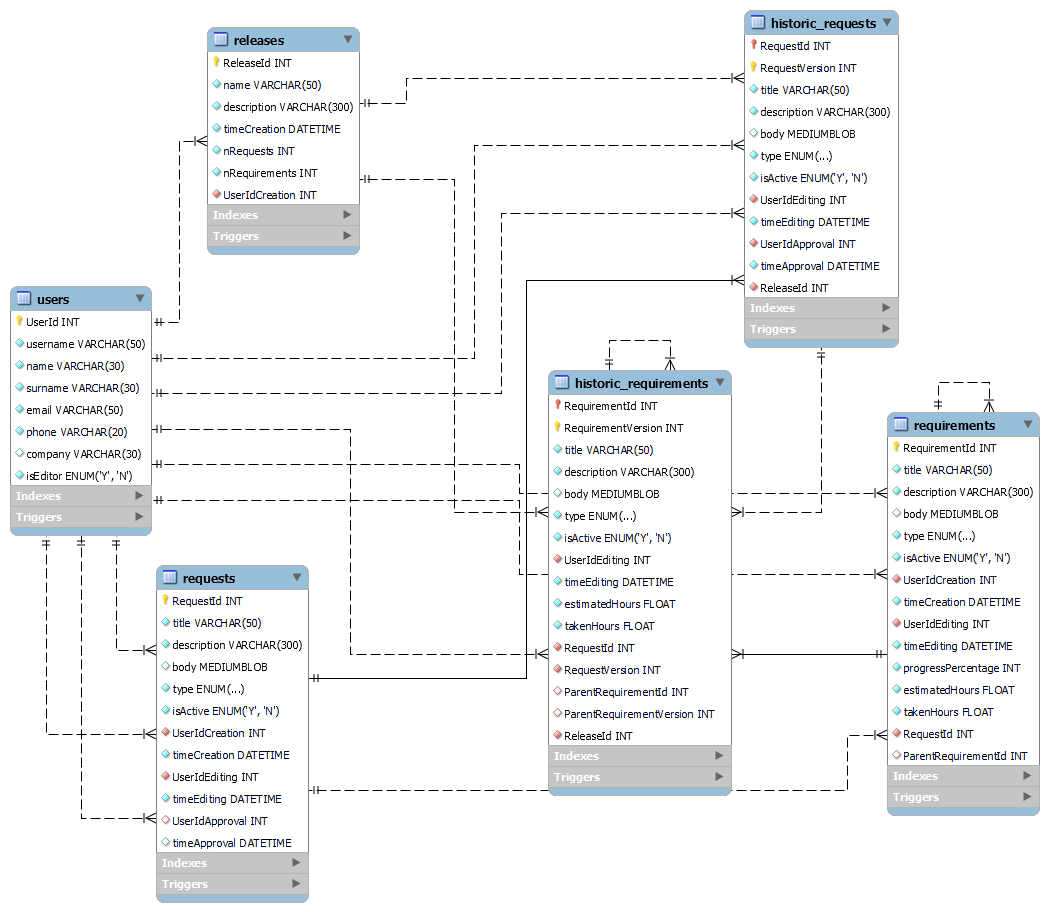
\includegraphics[width=\textwidth]{E-R logic}
\label{fig:ER_logic}
\end{figure}

\subsubsection*{Entity and Relationships Translation in Relations}

\textbf{USERS}(\underline{UserId}, username, name, surname, email, phone, company*, isEditor)\newline
\newline
NOTES:\newline
Unique(username)\newline
Unique(email)\newline
\newline
\textbf{RELEASES}(\underline{ReleaseId}, name, description, timeCreation, nRequests, nRequirements,
UserIdCreation: \textit{USERS})\newline
\newline
NOTES:\newline
Unique(name)\newline
\newline
\textbf{REQUESTS}(\underline{RequestId}, title, description, body*, type, isActive, UserIdCreation: \textit{USERS}, timeCreation,
UserIdEditing: \textit{USERS}, timeEditing, UserIdApproval*: \textit{USERS}, timeApproval*)\newline
\newline
NOTES:\newline
A constraint should make `UserIdApproval' and `timeApproval' to be both present or absent at the same time.\newline
\newline
\textbf{REQUIREMENTS}(\underline{RequirementId}, title, description, body*, type, isActive, UserIdCreation: \textit{USERS},
timeCreation, UserIdEditing: \textit{USERS}, timeEditing, progressPercentage, estimatedHours, takenHours,
RequestId: \textit{REQUESTS}, ParentRequirementId*: \textit{REQUIREMENTS})\newline
\newline
\textbf{HISTORIC\_REQUESTS}(\underline{RequestId}: \textit{REQUESTS}, \underline{RequestVersion}, title, description, body*, type,
isActive, UserIdEditing: \textit{USERS}, timeEditing, timeApproval, ReleaseId: \textit{RELEASES})\newline
\newline
\textbf{HISTORIC\_REQUIREMENTS}(\underline{RequirementId}: \textit{REQUIREMENTS}, \underline{RequirementVersion}, title,
description, body*, type, isActive, UserIdEditing: \textit{USERS}, timeEditing, estimatedHours, takenHours,
(RequestId, RequestVersion): \textit{HISTORIC\_REQUESTS},
(ParentRequirementId, ParentRequirementVersion)*: \textit{HISTORIC\_REQUIREMENTS}, ReleaseId: \textit{RELEASES})

\subsubsection*{Relations Analysis}

\paragraph{Attributes}
An attribute of a relation $A$ can be set in an instance with a value that is its domain $dom(A)$.
Let's consider $T = \{A_1, A_2, ..., A_n\}$ a set of attributes.

\paragraph{Tuples}
A tuple t on T is a function that maps for each $A_i \in T$ a value in $dom(A_i)$.

\paragraph{Schema of Relation}
A schema of relation on $T$ is defined by the name of the relation $R$ and a set of attributes $T$,
an it is denoted by $R(T)$. An extension of it can be denoted by $r$.

\paragraph{Functional Dependency}
A functional dependency (FD), considering a schema $R(T)$ and $X, Y \subseteq T$ with $X, Y \neq \emptyset$,
is defined as $X \rightarrow Y$ (X functionally determines Y) if:
$$
\forall \ t_1, t_2 \in r : t_1[X] = t_2[X] \Rightarrow t_1[Y] = t_2[Y]
$$
Note that FD is a feature of the $R(T)$ and not its extension $r$.

\paragraph{Trivial Functional Dependency}
A functional dependency is trivial if $Y \subseteq X$.

\paragraph{Super Key}
$K \subseteq T$ is a super-key of $R(T) \Leftrightarrow K \rightarrow T$.

\paragraph{Key}
A key is a super-key without subset of attributes that is another super-key.

\paragraph{Attributes and Keys}
Attributes can be:
\begin{enumerate}
    \item \textit{prime}: is part of at least one key in the schema.
    \item \textit{non-prime}: it is not part of any key in the schema.
\end{enumerate}

\paragraph{Normal Forms}
It was considered the following normal forms:
\begin{enumerate}
    \item First Normal Form (1NF):
    \begin{enumerate}
        \item A schema $R(T)$ is in 1NF if and only if the domain of each attribute contains only atomic values (simple,
              indivisible), and the value of each attribute in a tuple is a single value from the domain of that attribute.
    \end{enumerate}
    \item Second Normal Form (2NF):
    \begin{enumerate}
        \item A schema $R(T)$ with constraints $F$ is in 2NF if and only if every non-prime attribute depends entirely (not
              partially) on every candidate key of the schema, meaning there is no partial dependency of a non-prime attribute
              on a key.
    \end{enumerate}
    \item Third Normal Form (3NF):
    \begin{enumerate}
        \item A schema $R(T)$ with constraints $F$ is in 3NF if and only if every non-prime attribute does not depend transitively
              on any key, meaning there is no transitive dependency of a non-prime attribute on a key.
        \item Every relation can reach this level after modifications of splitting and/or merging.
    \end{enumerate}
    \item Boyce-Codd Normal Form (BCNF):
    \begin{enumerate}
        \item A schema $R(T)$ with constraints $F$ is in BCNF if and only if, for every non-trivial functional dependency
              $X \rightarrow Y$ defined on it, $X$ is a super-key of $R(T)$.
        \item It extends what seen till now to prime attributes.
        \item Some relationships cannot reach this level even after modifications of splitting and/or merging.
    \end{enumerate}
\end{enumerate}
All relations considered are in BCNF.

\chapter*{Deployment}
\addcontentsline{toc}{chapter}{Deployment}

\section*{MySQL Queries}
\addcontentsline{toc}{section}{MySQL Queries}

In this section the previously described \hyperref[subsec:ops]{operations} are translated into MySQL queries.

\hyperref[subsubsec:op1]{Subscribe a new user} operation query described in \autoref{lst:mysqlquery1}.

\begin{lstlisting}[language=MySQL, caption={\texorpdfstring{\hyperref[subsubsec:op1]{op. 1}}{op. 1}}, label={lst:mysqlquery1}]
    -- UserId was set as AUTO_INCREMENT, so it can be omitted here
    INSERT INTO `USERS`
        (`username`, `name`, `surname`,
         `email`, `phone`, `company`,
         `isEditor`)
    VALUES
        (?, ?, ?, ?, ?, ?, ?);
\end{lstlisting}

\hyperref[subsubsec:op2]{View a request} operation query described in \autoref{lst:mysqlquery2}.

\begin{lstlisting}[language=MySQL, caption={\texorpdfstring{\hyperref[subsubsec:op2]{op. 2}}{op. 2}}, label={lst:mysqlquery2}]
    SELECT *
    FROM `REQUESTS`
    WHERE `RequestId` = ?;
\end{lstlisting}

\hyperref[subsubsec:op3]{Create a request} operation query described in \autoref{lst:mysqlquery3}.

\begin{lstlisting}[language=MySQL, caption={\texorpdfstring{\hyperref[subsubsec:op3]{op. 3}}{op. 3}}, label={lst:mysqlquery3}]
    INSERT INTO `REQUESTS`
        (`title`, `description`, `type`,
         `isActive`, `UserIdCreation`,
         `UserIdEditing`, `timeEditing`)
    VALUES
        (?, ?, ?, ?, ?, ?, NOW());
\end{lstlisting}

\hyperref[subsubsec:op4]{Update a request} operation query described in \autoref{lst:mysqlquery4}.

\begin{lstlisting}[language=MySQL, caption={\texorpdfstring{\hyperref[subsubsec:op4]{op. 4}}{op. 4}}, label={lst:mysqlquery4}]
    UPDATE `REQUESTS`
    SET `title` = ?,
        `description` = ?,
        `body` = ?,
        `type` = ?,
        `isActive` = ?,
        `UserIdEditing` = ?,
        `timeEditing` = NOW()
    WHERE `RequestId` = ?;
\end{lstlisting}

\hyperref[subsubsec:op5]{Approve a request} operation query described in \autoref{lst:mysqlquery5}.

\begin{lstlisting}[language=MySQL, caption={\texorpdfstring{\hyperref[subsubsec:op5]{op. 5}}{op. 5}}, label={lst:mysqlquery5}]
    UPDATE `REQUESTS`
    SET `UserIdApproval` = ?,
        `timeApproval` = NOW(),
        `UserIdEditing` = ?,
        `timeEditing` = NOW()
    WHERE `RequestId` = ?;
\end{lstlisting}

\hyperref[subsubsec:op6]{View a requirement} operation query described in \autoref{lst:mysqlquery6}.

\begin{lstlisting}[language=MySQL, caption={\texorpdfstring{\hyperref[subsubsec:op6]{op. 6}}{op. 6}}, label={lst:mysqlquery6}]
    SELECT *
    FROM `REQUIREMENTS`
    WHERE `RequirementId` = ?;
\end{lstlisting}

\hyperref[subsubsec:op7]{Create a requirement} operation query described in \autoref{lst:mysqlquery8}.

\begin{lstlisting}[language=MySQL, caption={\texorpdfstring{\hyperref[subsubsec:op7]{op. 7}}{op. 7}}, label={lst:mysqlquery7}]
    INSERT INTO `REQUIREMENTS`
        (`title`, `description`, `type`,
         `isActive`, `UserIdCreation`,
         `UserIdEditing`, `timeEditing`
         `RequestId`, `ParentRequirementId`)
    VALUES
        (?, ?, ?, ?, ?, ?, NOW(), ?, ?);
\end{lstlisting}

\hyperref[subsubsec:op8]{Update a requirement} operation query described in \autoref{lst:mysqlquery8}.

\begin{lstlisting}[language=MySQL, caption={\texorpdfstring{\hyperref[subsubsec:op8]{op. 8}}{op. 8}}, label={lst:mysqlquery8}]
    UPDATE `REQUIREMENTS`
    SET `title` = ?,
        `description` = ?,
        `body` = ?,
        `type` = ?,
        `isActive` = ?,
        `UserIdEditing` = ?,
        `timeEditing` = NOW(),
        `progressPercentage` = ?,
        `estimatedHours` = ?,
        `takenHours` = ?
    WHERE `RequestId` = ?;
\end{lstlisting}

\hyperref[subsubsec:op9]{Disable a requirement} operation query described in \autoref{lst:mysqlquery9}.

\begin{lstlisting}[language=MySQL, caption={\texorpdfstring{\hyperref[subsubsec:op9]{op. 9}}{op. 9}}, label={lst:mysqlquery9}]
    UPDATE `REQUIREMENTS`
    SET `isActive` = ?,
        `UserIdEditing` = ?,
        `timeEditing` = NOW(),
    WHERE `RequestId` = ?;
\end{lstlisting}

\hyperref[subsubsec:op10]{View a release} operation query described in \autoref{lst:mysqlquery10}.

\begin{lstlisting}[language=MySQL, caption={\texorpdfstring{\hyperref[subsubsec:op10]{op. 10}}{op. 10}}, label={lst:mysqlquery10}]
    SELECT *
    FROM `RELEASES`
    WHERE `ReleaseId` = ?;
\end{lstlisting}

\hyperref[subsubsec:op11]{Create a release} operation query described in \autoref{lst:mysqlquery11}.

\begin{lstlisting}[language=MySQL, caption={\texorpdfstring{\hyperref[subsubsec:op11]{op. 11}}{op. 11}}, label={lst:mysqlquery11}]
    INSERT INTO `RELEASES`
        (`name`, `description`, `UserIdCreation`)
    VALUES
        (?, ?, ?);
\end{lstlisting}

\hyperref[subsubsec:op12]{Show requirements and requests relative to a specific release} operation query described in
\autoref{lst:mysqlquery12}.

\begin{lstlisting}[language=MySQL, caption={\texorpdfstring{\hyperref[subsubsec:op12]{op. 12}}{op. 12}}, label={lst:mysqlquery12}]
    SELECT
        h_requests.*,
        h_r.*
    FROM
        `RELEASES` releases,
        `HISTORIC_REQUESTS` h_requests,
        `HISTORIC_REQUIREMENTS` h_r
    WHERE
        releases.`ReleaseId` = h_requests.`ReleaseId` AND
        releases.`ReleaseId` = h_r.`ReleaseId`;
    -- is equivalent to
    SELECT
        h_requests.*,
        h_r.*
    FROM
        `RELEASES` releases,
    INNER JOIN `HISTORIC_REQUESTS` h_requests
        ON requests.`ReleaseId` = releases.`ReleaseId`
    INNER JOIN `HISTORIC_REQUIREMENTS` h_r
        ON h_r.`ReleaseId` = h_r.`ReleaseId`;
\end{lstlisting}

\hyperref[subsubsec:op13]{View single requirement history} operation query described in \autoref{lst:mysqlquery13}.

\begin{lstlisting}[language=MySQL, caption={\texorpdfstring{\hyperref[subsubsec:op13]{op. 13}}{op. 13}}, label={lst:mysqlquery13}]
    SELECT
        h_r.*
    FROM
        `REQUIREMENTS` r,
        `HISTORIC_REQUIREMENTS` h_r
    WHERE
        r.`RequirementId` = h_r.`RequirementId` AND
        r.`RequirementId` = ?;
\end{lstlisting}

\hyperref[subsubsec:op14]{Obtain an average of the progress time relative to a branch of the requirements tree} operation
query described in \autoref{lst:mysqlquery14}.

\begin{lstlisting}[language=MySQL, caption={\texorpdfstring{\hyperref[subsubsec:op14]{op. 14}}{op. 14}}, label={lst:mysqlquery14}]
    -- Common Table Expressions are supported from MySQL 8
    WITH RECURSIVE `RequirementTree` AS (
        -- Anchor member: Select the starting node (the root of the branch)
        SELECT *
        FROM `REQUIREMENTS`
        WHERE `RequirementId` = ? -- Replace with the ID of the root
        UNION ALL
        -- Recursive member: Select all children of the current level
        SELECT r.*
        FROM `REQUIREMENTS` r
        INNER JOIN `RequirementTree` rt ON r.`ParentRequirementId` = rt.`RequirementId`
    )
    -- Final selection: Sum up the values from the CTE
    SELECT
        SUM(`progressPercentage`) AS `totalProgressPercentage`,
        SUM(`estimatedHours`) AS `totalEstimatedTime`,
        SUM(`takenHours`) AS `totalTakenTime`
    FROM `RequirementTree`;
\end{lstlisting}

\section*{Application}
\addcontentsline{toc}{section}{Application}

It was chosen a C\# .NET Core 8.0 application running on Windows with Windows Forms GUI.
As anticipated with the queries the database is MySQL.

Following this report philosophy it was adopted a database first approach.
So at first the \nameref{chap:analysis} was written, with: requirements, conceptual and logical design, and then the
implementation started.
A file named `ReM.sql' was used as a script, partially derived from design and partially handwritten, to create schema (database)
and tables in MySQL. It includes features to avoid illegal situations using checks and triggers, except for historic data that
should be modified only behind the scenes in a real application.

So as to map data from MySQL to .NET Core 8.0 it was chosen to use Entity Framework Core.
In particular with the process of `Scaffolding'
\footnote{\url{https://dev.mysql.com/doc/connector-net/en/connector-net-entityframework-core-scaffold-example.html}}
it was possible to map directly the `ReM' schema from MySQL to .NET Core 8.0 classes.

% \appendix

% \printbibliography

\end{document}